%##########################  CHAPER 6: APPLICATION  #######################

\chapter{Entwicklung der Anwendung}\label{kap:application}

Dieses Kapitel beschreibt die Entwicklung der Anwendung, als 
autonomes System welches auf dem Raspberry Pi läuft, 
Bilder über eine infrarotfähige Kamera aufnimmt und diese
auf dem Neural Compute Stick 2 mit dem trainierten Modell 
inferiert.
Desweiteren wird die Implementierung der verbindugn zu einem 
Host Pc beschrieben.


%-------------------------  SECTION 1: AUFBAU  ------------------------
\section{Aufbau/Hardware}\label{sec:aufbau}

Im folgenden werden die zur Realisierung der Anwendung verwendeten 
Komponenten erläutert.

\subsection*{Raspberry Pi}
Der Anwendungs Code läuft auf dem Raspberry Pi. 
Der Neural Compute Stick 2 wird über eine USB Schnittstelle verbunden.


\begin{figure}[H]
    \centering
    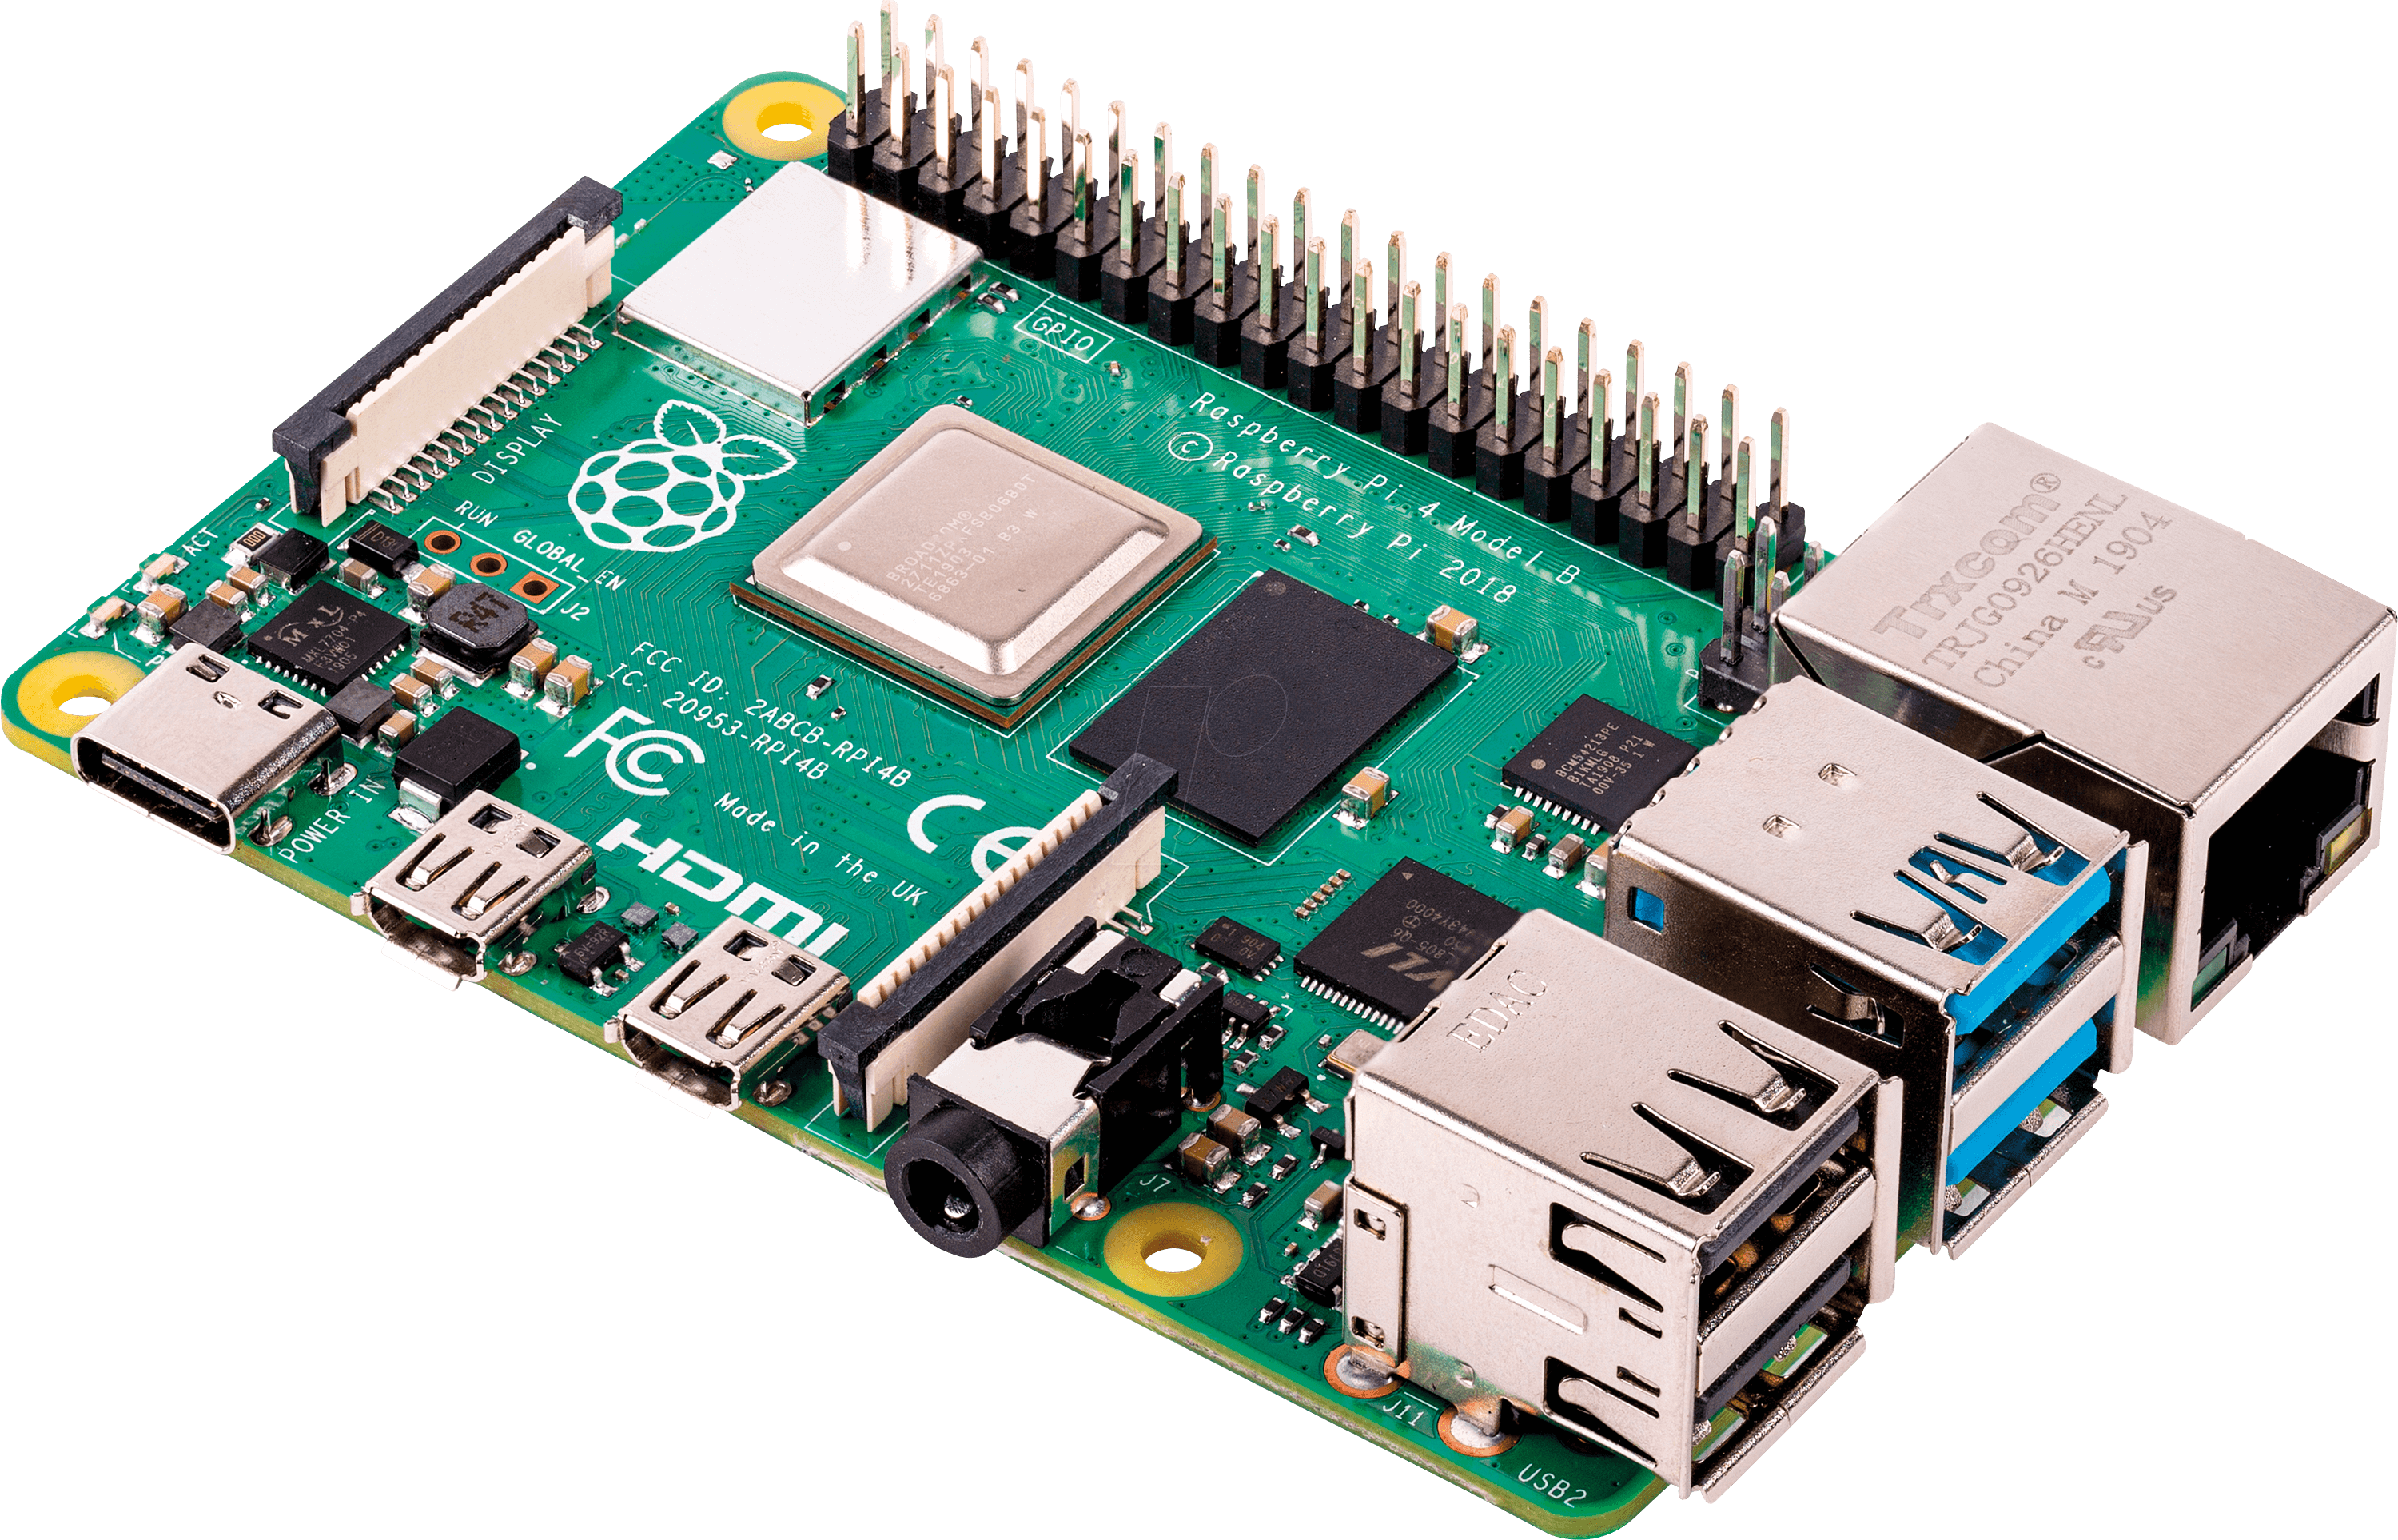
\includegraphics[width=6cm]{./Bilder/raspberrypi_4.png}
    \caption{Raspberry Pi 4}
    \label{img:raspberrypi}
\end{figure}



\subsection*{Kamera}
Verwendet wurde ein Raspberry Pi Kamera Modul mit 5MP OV5647 Sensor 
und automatschem umschalten der Infrarot Funktion der Marke 
Longrunner verwendet.
%https://www.amazon.de/gp/product/B07R4JH2ZV/ref=ppx_yo_dt_b_asin_title_o01_s00?ie=UTF8&psc=1
Dieses verfügt zusätzlich über zwei Infrarot LEDs, mit 850 nm wellenlänge.

\begin{figure}[H]
    \centering
    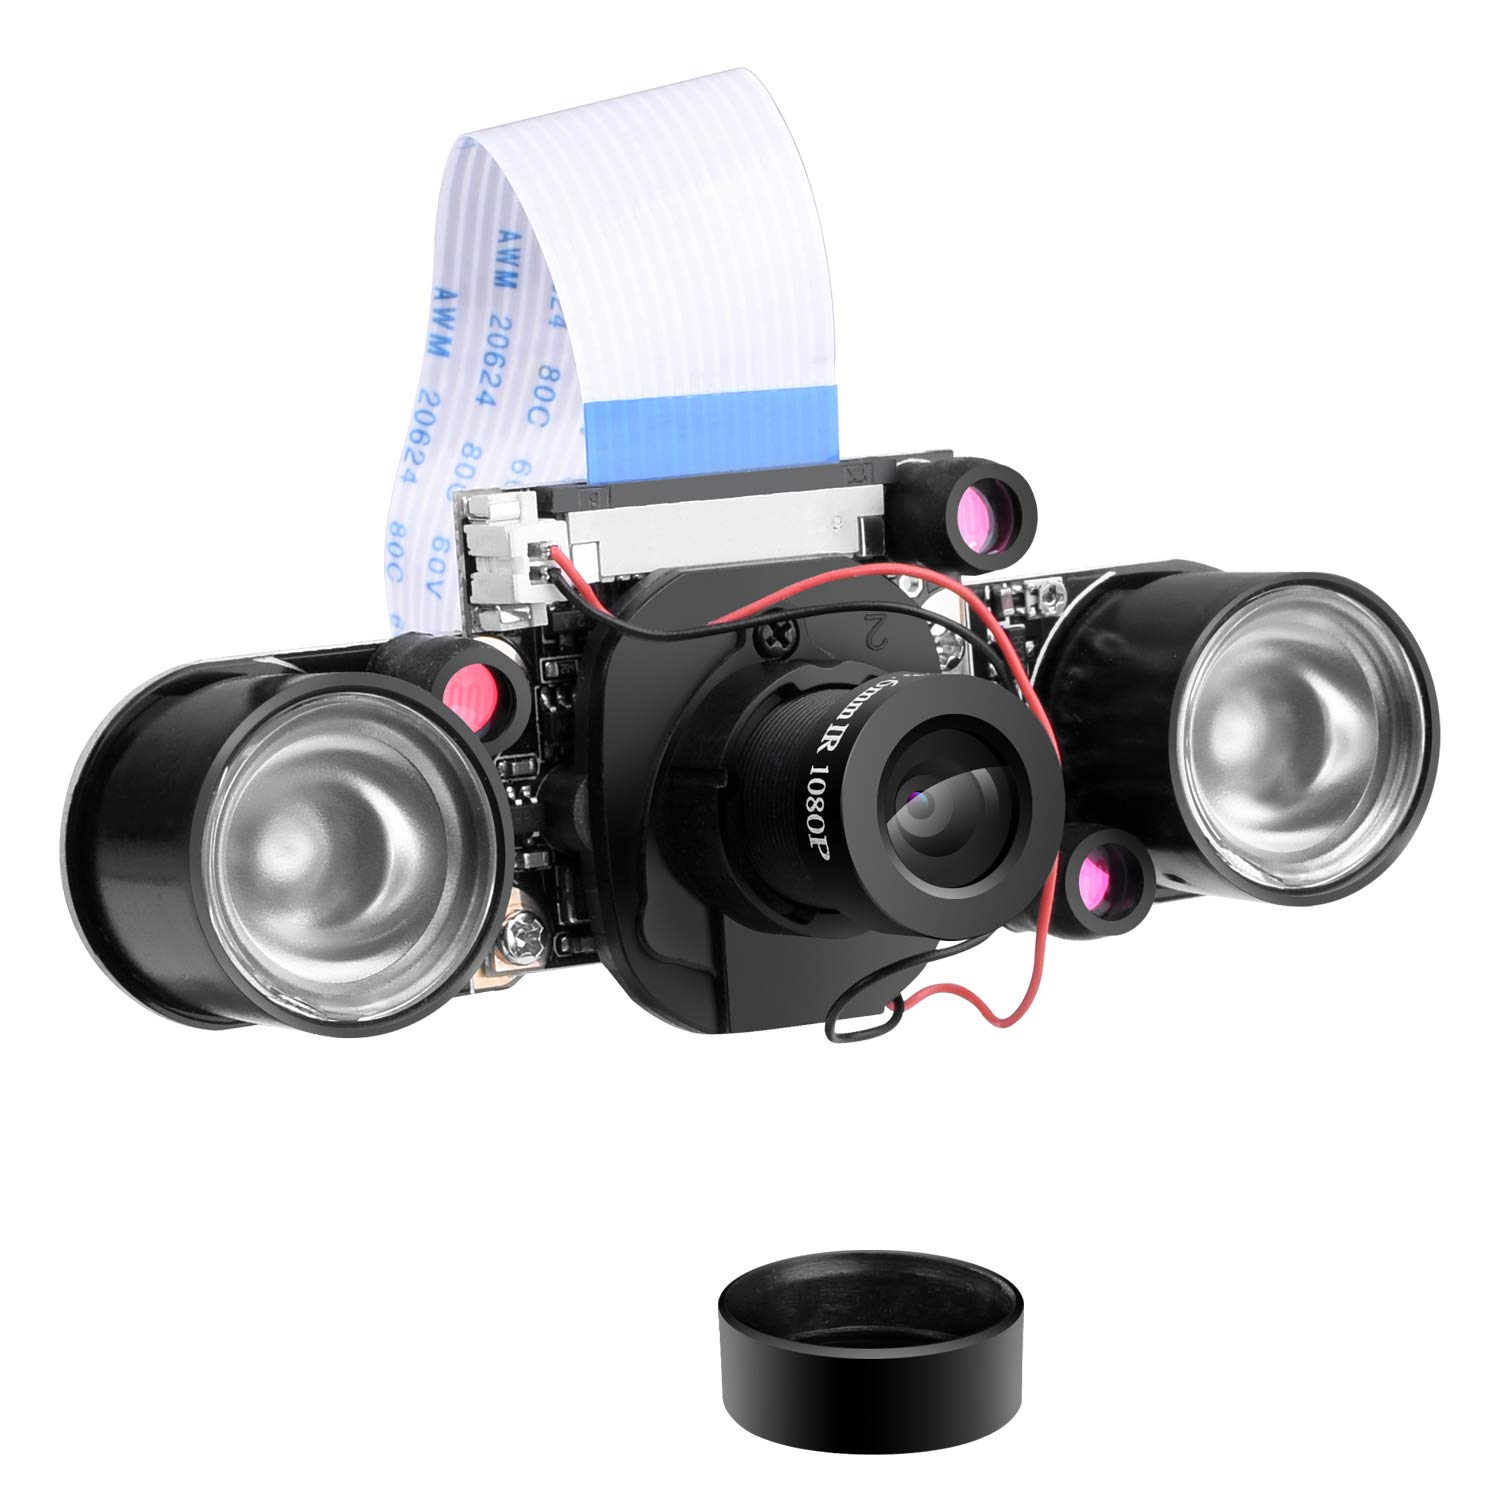
\includegraphics[width=0.35\textwidth]{longrunner.jpg}
    \caption{Longruner for Raspberry Pi 4 Camera Kamera Module}
    \label{fig:rpicam}
\end{figure}

Für das Umschalten in den Infrarot Modus, wird der Infrarot Filder, welcher sich 
für normale Aufnahmen vor der Linse befindet entfern, was über einen magnetschalter 
der mit einem Helligkeitssensor getriggert wird erfolg.

 

\subsection*{sonstiges}
\begin{itemize}
    \item Internet Stick%https://www.amazon.de/gp/product/B00HSZEY34/ref=ppx_yo_dt_b_asin_title_o00_s00?ie=UTF8&psc=1
    \item Hülle
    \item Powerbank
\end{itemize}

\section{Implementierung/Software}

in Python, 3 Programme, main, inferenz, connection

hier gesammt programm beschreiben mit entweder 
Klassendiagramm oder Pseudo code.

\subsection*{Inferenz}

heir die implementierung des infer scripts (mit non blocking, 
buffer, motion)


Um nicht durchgehend die Input Frames welche die Kamera liefert inferieren zu 
müssen, wurde mithilfe der Library OpenCV ein bewegungserkennung 
implementiert. Diese speichert bei start der Anwendung ein Frame 
als Refernz ab, und kann damit alle weiteren Input frames vergleiche, 
indem der Abstand der einzelnen Pixel werte berechnet und gemittelt wird.


%Asynchrone inferenz
%https://docs.openvinotoolkit.org/latest/_demos_python_demos_object_detection_demo_ssd_async_README.html



\begin{algorithm}[H]
    \caption{Asynchrone Inferenz}
    \begin{algorithmic}
        \WHILE{\TRUE}

        \STATE capture Frame
        \IF{frame has moton}
            \STATE $buffer \leftarrow 1 / frmae$
        \ENDIF

        \FOR{$inferReq = 0$ to $maxReq$}
        \STATE status = exec.req(inferReq).wait(0)
        \IF {status == done}
            \STATE ROIs = exec.req(inferReq).output
            \STATE results.add(ROIs, frame[inferReq])
        \ENDIF

        \ENDFOR

        \ENDWHILE

    \end{algorithmic}
\end{algorithm}



\subsection*{Connection}

hier prinzip remote Proxy verbindung über SSH und SCP Protokol erklären
sowie implementierung mit remote it api und scp command.





